\subsection*{Problem B2}

    The linearisation of the system was tested by writing simulating both systems in Python. The implementation of the simulations can be found \href{https://github.com/drlim2u/ELE2024-Control-Coursework/blob/4dc7e6f918fce68ee3aef799fe1dba15ea789481/PartB.py#L44}{here}.

    \begin{figure}[H]
        \centering
        \includegraphics[width=0.6\linewidth]{figures/problem_b2_a.eps}
        \caption{Three plots of the simulation of the non-linear system with the \(x\) position, \(\dot{x}\) and \(I\) of the ball in respect to time.}
        \label{fig:problem_b2_a}
    \end{figure}
    
    \begin{figure}[H]
        \centering
        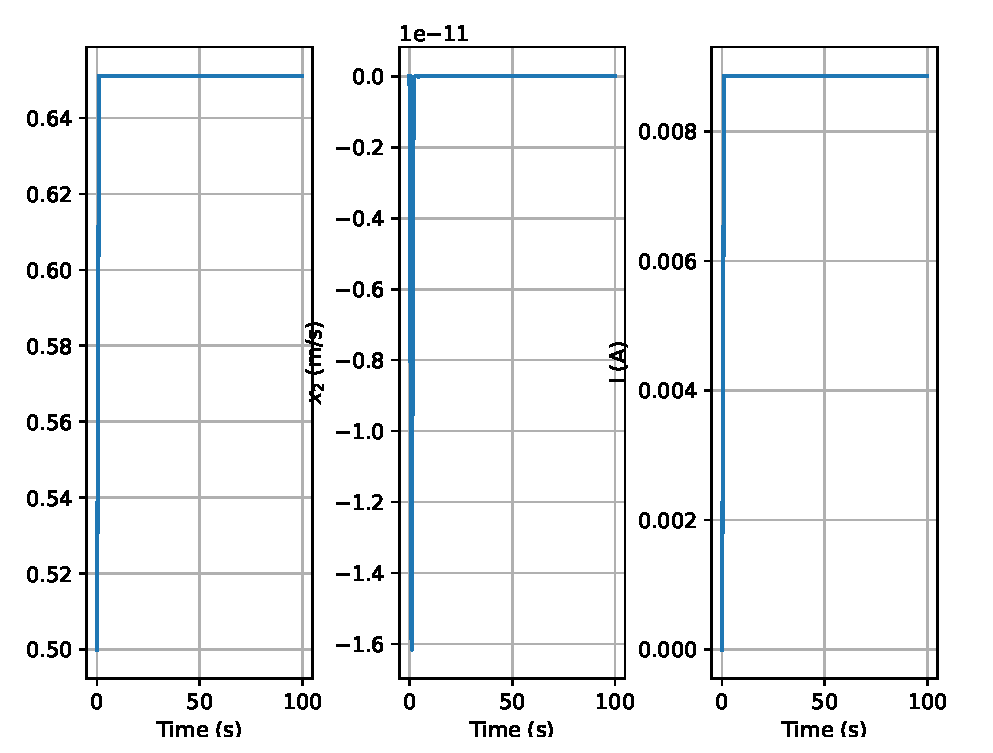
\includegraphics[width=0.6\linewidth]{figures/problem_b2_b.eps}
        \caption{Three plots of the simulation of the linearised system with the \(x\) position, \(\dot{x}\) and \(I\) of the ball in respect to time.}
        \label{fig:problem_b2_b}
    \end{figure}
    
    As can be seen in both Figure \ref{fig:problem_b2_a} and Figure \ref{fig:problem_b2_b} both simulations showed stable systems. However the non-linear system shown in Figure \ref{fig:problem_b2_a} does not behave close to the equilibrium point of the linearised system shown in Figure \ref{fig:problem_b2_b}. The non-linear system shows an equilibrium point of \(x_1\) at around 0.42m whereas the linearised system shows that the equilibrium point of \(x_1\) is around 0.65m. It can therefore be determined, assuming that the simulation was programmed correctly, that there is an error in the linearisation. It is believed that this issue comes specifically from the linearisation of \(\dot{I}\).
